\section{Obrzęd Komunii Św.}

    \begin{itemize}
     \item \ii~ zmienia szaty - asystuje \cc1
     \item \ii~ zanosi korporał na ołtarz w towarzystwie \cc1 i \cc2
     \item \aa1 i \aa2 ustawiają się przed stopniami ołtarza i wraz z \oo~, \cc1, \cc2 i \ii~ procesyjnie udają się to ołtarza przechowywania 
     \item podczas powrotu procesji do ołtarza, \cc1 i \cc2 uderzają kołatką, a wszyscy ministranci klęczą
     \item po dojściu do stopni ołatarza \oo~ odchodzi na bok, \aa1 i \aa2 odkładają akolitki na ołtarzu, a \cc1, \cc2 i \ii~ podchodzą do ołarza
     
     \begin{figure}[h]
     \centering
        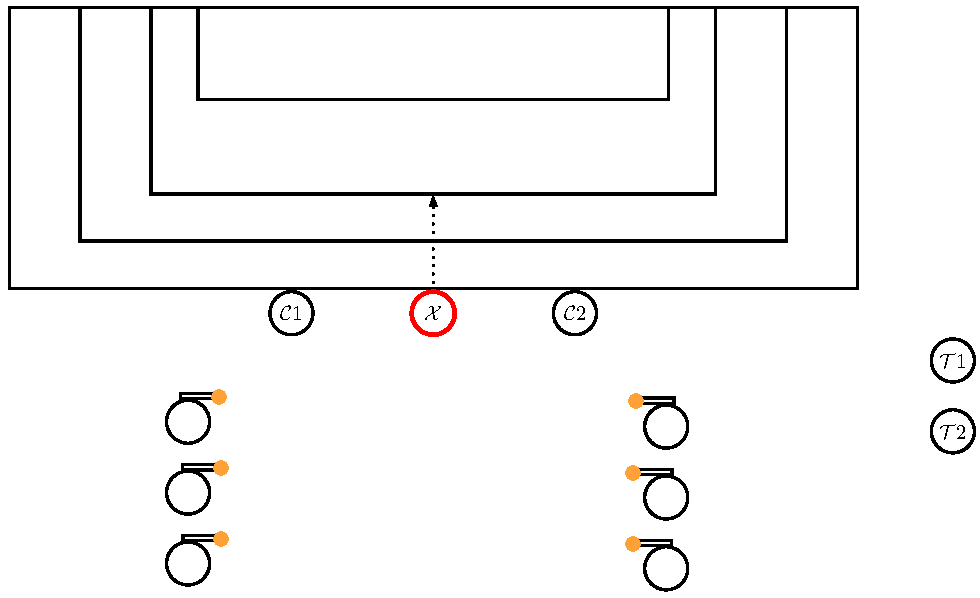
\includegraphics[scale=0.6]{Piatek/NSakrament.pdf}
     \end{figure}
     
     \item przy ołtarzu \cc2 odbiera welon, po czym przyklęka i idzie na swoje miejsce
     \item wszyscy ministranci wstają; w odpowiednim momencie za \ii~ odmawiają \textit{Pater noster}
     \item na znak \cc1 ministranci ustawiają się parami na posadzce do przyjęcia Komunii i na kolejny znak - klękają
     \item w tym czasie \aa1 (z obrusem komunijnym) i \aa2 klękają twarzami do siebie na najwyższym stopniu ołtarza
     \item \cc1 rozpoczyna \textit{Confiteor}, do którego dołączają się pozostali
     \item po \textit{Indulgentiam...} \aa1 i \aa2 rozciągają obrus komunijny między sobą
     \item pierwsi do Komunii przystępują ministranci od pateny i świeczki sanctusowej; zaraz po jej przyjęciu asystują \ii~
     \item do Komunii ministranci przystępują w następujący sposób (więcej: \hyperref[komunia]{patrz Dodatek}):
     
      \begin{enumerate}[leftmargin=1cm]
       \item para przyklęka na posadzce równocześnie z poprzedzającą ją parą
       \item po wejściu na stopnie ołtarza, klęka na najwyższym stopniu
       \item przyjąwszy Komunię, przyklęka w miejscu i udaje się na swoje miejsce
      \end{enumerate}
    
     \item po przyjęciu Komunii św. przez ministrantów, \aa1 i \aa2 wstają i udają się z obrusem komunijnym do balasek; razem z nimi przechodzą \cc1 i \cc2
     \item po skończonej Komunii wiernych, \aa1 i \aa2 składają obrus komunijny i odkładają na kredensji i przy niej pozostają
     \item wszyscy wstają, gdy zostanie schowany Najświętszy Sakrament i pozostają w tej pozycji
     \item gdy \ii~ oczyści patenę, zabiera ją \aa1; korporał nie jest chowany!
     \item \ii~ śpiewa trzy modlitwy po komuni; po nich \cc2 zamyka i ściąga z ołtarza mszał
     \item \ii~ udaje się do sedilii i zmienia szaty - asystuje \cc1
    \end{itemize}

